\indent \section{Проблематика развития синтаксического парсера русского языка}
В главе рассмотрены основные термины и понятия по теме работы, предложена технология поиска необходимой информации, произведен анализ аналогов, выбраны критерии для оценки аналогов и их оценка по выделенным критериям, выбран прототип, сформулированы цели и задачи диссертации.

\subsection{Основные термины и понятия}
Естественный язык --- язык племени, народа, нации, возникающий и развивающийся в данном этническом сообществе, в минимальной степени испытывающий сознательное воздействие, передающийся из поколения в поколение естественным путем \cite{academica_nl}.

Обработка естественного языка --- область компьютерных наук, искуственного интеллекта и лингвистики, изучающая взаимодействие между компьютерами и человеческими (естественными языками) \cite{wiki_nlp}.

Парсинг (синтаксический парсинг) --- процесс анализа строк символов на естественном или компьютерном языке в соответствии с правилами формальной грамматики \cite{wiki_parsing}.

Формальная грамматика --- множество правил продукции для строк формального языка, описывающих формирование строк из алфавита формального языка, соответствующих синтаксису этого языка \cite{wiki_fg}.

Локализация --- переработка существующего программного продукта с целью использования его в странах с другим языком \cite{academica_loc}.

Машинное обучение --- процесс, в результате которого машина (компьютер) способна показывать поведение, которое в неё не было явно заложено (запрограммировано) \cite{samuel}.

Semantic Web (семантическая паутина) --- инициатива World Wide Web Consortium по включению семантического содержимого в веб-страницы, структурированию современного веб-пространства на основе RDF \cite{wiki_semantic_web}.

Resource description framework (среда описания ресурса) --- это разработанная консорциумом Всемирной паутины модель для представления данных, в особенности --- метаданных, представляющая утверждения о ресурсах в виде, пригодном для машинной обработки \cite{wiki_rdf}. 

Онтология --- формальное представление знания в виде множества понятий и отношений между ними \cite{wiki_ont}.

\subsection{Литературно-аналитический обзор по теме работы}
Далее рассмотрена технология поиска информации по теме, предъявлены требования к аналогам, сформированы критерии их сравнения, описана технология выбора прототипа.

\subsubsection{Технология поиска информации}
Отбор аналогов осуществлялся в процессе поиска по следующим направлениям:
\begin{list}{\labelitemi}{\leftmargin=1.5cm}
	\item методы синтаксического парсинга (синтаксический парсинг, алгоритмы парсинга, формальные грамматики);
	\item методы синтаксического парсинга русского языка (сужение предыдущего направления применительно к русскому языку);
	\item синтаксические парсеры русского и английского языка (конкретные реализации, технические показатели и методы, лежащие в их основе).
\end{list}

Поиск производился преимущественно в сети Интернет с использованием алгоритма, представленного на рисунке \ref{fig:searchalg}

\begin{figure}[H]
	\centering
		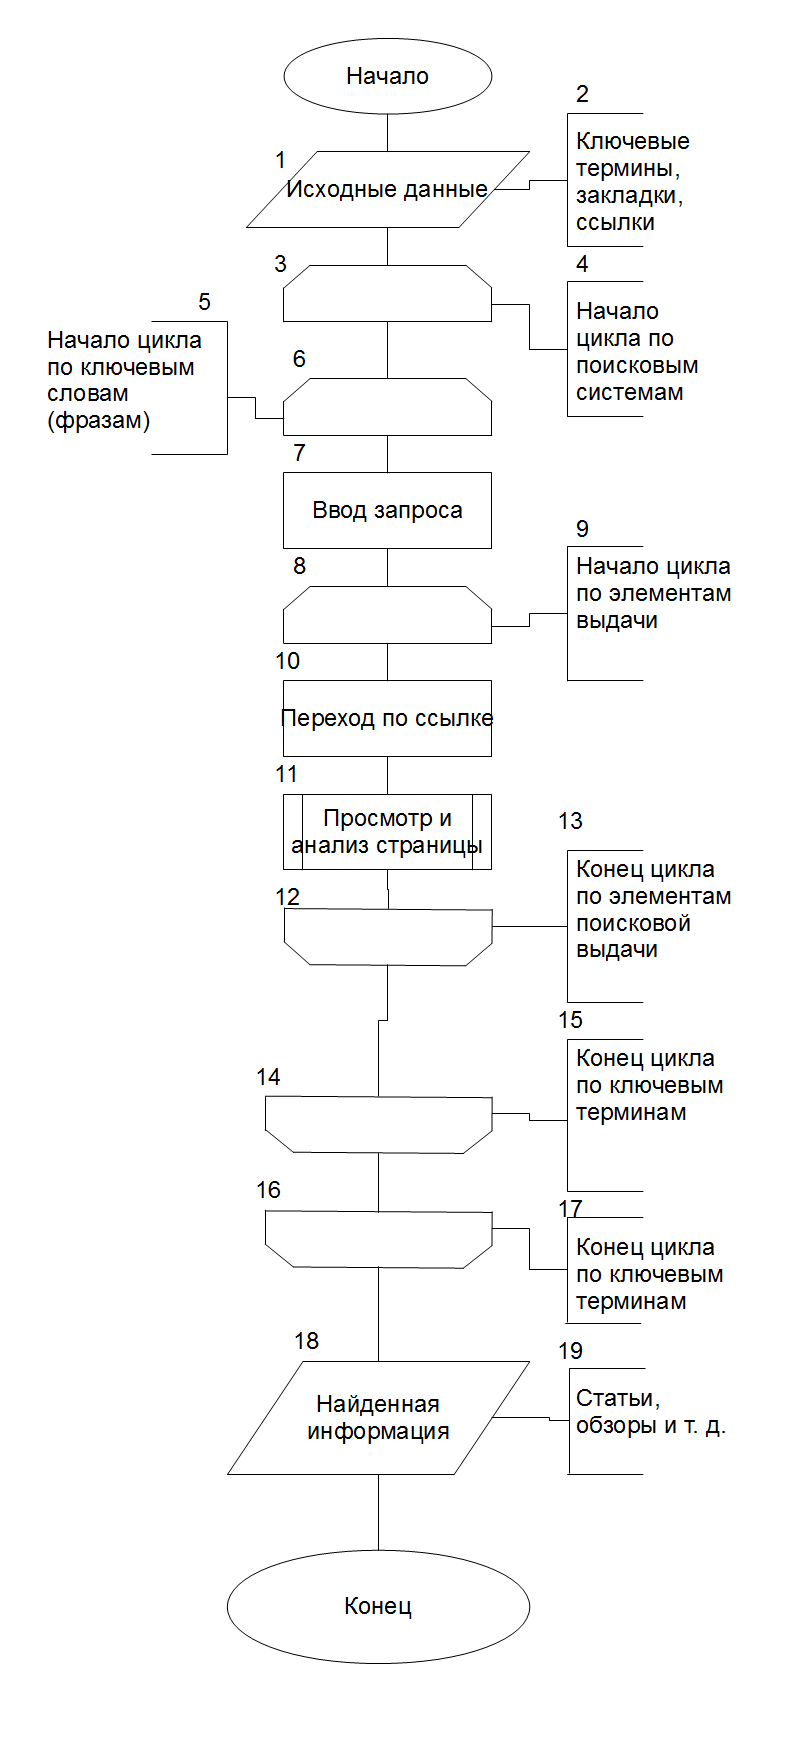
\includegraphics[scale=1.0]{images/searchalg.png}
	\caption{\small Алгоритм поиска информации в Интернете}
	\label{fig:searchalg}
\end{figure}

В приведённом на рисунке \ref{fig:searchalg} алгоритме использовались поисковые машины Google \cite{google}, Bing \cite{bing} и реже Yandex \cite{yandex}.

\subsubsection{Формирование требований к синтаксическому парсеру}
Выделение аналогов среди найденного производилось на основании максимального соответствия следующим предъявляемым к синтаксическим парсерам требованиям:
\begin{list}{\labelitemi}{\leftmargin=1.5cm}
	\item синтаксический парсер должен быть точным (минимальное число ошибок в результирующем дереве разбора, максимально корректное разрешение грамматически неоднозначных ситуаций) --- A;
	\item алгоритм синтаксического анализа должен быть эффективен (минимальная временная сложность алгоритма и сложность алгоритма по памяти, минимальное потребление памяти и процессорной мощности, максимальный потенциально возможный объём анализируемого текста) --- S;
	\item рассматриваемый аналог должен быть совместим с русским языком (минимальная степень специфичности грамматики по отношению к используемому языку, возможность реализовать формальную грамматику для русского языка на основе уже используемой парсером или наличие готовой) --- LS;
	\item входная информация должна быть в минимальной степени формализована (рассматриваемый аналог не должен требовать от входной информации предварительной обработки иными средствами естественноязыкового анализа) --- V.
\end{list}

\subsubsection{Критерии оценки аналогов}
Приведённые выше требования положены в основу четырёх критериев кортежной модели сравнения и оценки аналогов:\\
O = <A, S, LS, V; R>\\
где O --- интегральная оценка аналога, A --- критерий точности разбора, S --- критерий эффективности алгоритма, LS --- критерий простоты локализации грамматики, V --- критерий степени формализации входной информации, R --- матрица связи.

Методы оценки по выделенным критериям следующие:
\begin{list}{\labelitemi}{\leftmargin=1.5cm}
	\item A --- объективная нормированная процентная шкала, за нуль отсчёта взят минимальный показатель;
	\item S --- дискретная шкала, чем выше график производной функции сложности алгоритма, тем ниже оценка;
	\item LS --- дискретная шкала: 0.0 --- локализация грамматики невозможна, 0.25 --- для локализации необходима полная переработка грамматики, 0.50 --- достаточно изменить правила грамматики и провести машинное обучение, 0.75 --- достаточно отредактировать правила грамматики, 1.0 --- существует полноценная формальная грамматика русского языка;
	\item V --- дискретная шкала: 0.0 --- информация в виде метаданных, 0.50 --- информация в виде предварительно размеченного текста, 1.0 --- информация в виде необработанного текста.
\end{list}

Формула расчёта оценки аналога:

O \(= \alpha(A)*A + \alpha(S)*S + \alpha(LS)*LS + \alpha(V)*V\)\\
где 
\(\sum_{i=1}^{n} \alpha_i = 1\), \(\alpha_i\) --- весовой коэффициент соответствующего критерия, n --- количество критериев.

Найдём весовые коэффициенты методом попарного сравнения критериев Томаса Саати \cite{tsaati}. 
Будем использовать шкалу от 1 до 9, где: 
\begin{list}{\labelitemi}{\leftmargin=1.5cm}
  \item 1 --- равенство;
  \item 2 --- промежуточное значение;
  \item 3 --- слабое превосходство;
  \item 4 --- промежуточное значение;
  \item 5 --- сильное превосходство;
  \item 6 --- промежуточное значение;
  \item 7 --- значительное превосходство;
  \item 8 --- промежуточное значение;
  \item 9 --- абсолютное превосходство.
\end{list}
Матрица попарного сравнение представлена в таблице \ref{tab:crit}.

\begin{table}[H]
\centering
\caption{Матрица попарного сравнения критериев}
{\small 
\begin{tabu}to \textwidth{ | X[c] | X[c] | X[c] | X[c] | X[c] | X[c] | X[c] | }
	\hline
          & A   & S   & LS  & V & Среднее & Вес  \\ \hline
	A     & 1   & 3   & 4   & 7 & 3.75    & 0.51 \\
	S     & 1/3 & 1   & 3   & 5 & 2.33    & 0.31 \\
	LS    & 1/4 & 1/3 & 1   & 2 & 0.90    & 0.12 \\
	V     & 1/7 & 1/5 & 1/2 & 1 & 0.43    & 0.06 \\ \hline
	Сумма &     &     &     &   & 7.41    & 1.00 \\
	\hline
\end{tabu}
}
\label{tab:crit}
\end{table}

\subsubsection{Обзор найденных аналогов}

\subsubsection{Выбор прототипа}
Выделенные в требованиях характеристики для найденных аналогов были определены и сведены в таблице \ref{tab:obj}.

\begin{table}[H]
\centering
\caption{Результат объективной оценки аналогов по критериям}
{\small 
\begin{tabu}to \textwidth{ | X[c] | X[c] | X[c] | X[c] | X[c] | }
	\hline
    Аналог/Критерий & A    & S                & LS   & V   \\ \hline
	BLA                      & 75.9 & \(O(n^3)\)       & 0.50 & 1.0 \\ \hline
	SP                       & 72.8 & \(O(n^3*|G|^2)\) & 0.50 & 1.0 \\ \hline
	RG                       & 78.1 & \(O(n^5)\)       & 0.50 & 1.0 \\ \hline
	CYK                      & 66.6 & \(O(n^3*|G|)\)   & 0.75 & 0.5 \\ \hline
	IOA                      & 56.0 & \(O(n^3)\)       & 0.50 & 1.0 \\ \hline
	EA                       & 78.0 & \(O(n^3)\)       & 0.75 & 0.5 \\ \hline
	LGP                      & 73.0 & \(O(n^3)\)       & 1.00 & 1.0 \\ 
	\hline
\end{tabu}
}
\label{tab:obj}
\end{table}

С учётом приведённой ранее системы выставления оценок, объективные показатели были переведены в значения на соответствющих шкалах и нормированы. Результат представлен в таблице \ref{tab:scales}.

\begin{table}[H]
\centering
\caption{Результат нормированной оценки аналогов по шкалам критериев}
{\small 
\begin{tabu}to \textwidth{ | X[c] | X[c] | X[c] | X[c] | X[c] | }
	\hline
    Аналог/Критерий          & A    & S     & LS   & V   \\ \hline
	BLA                      & 0.97 & 1.00  & 0.50 & 1.0 \\ \hline
	SP                       & 0.93 & 0.50  & 0.50 & 1.0 \\ \hline
	RG                       & 1.00 & 0.00  & 0.50 & 1.0 \\ \hline
	CYK                      & 0.85 & 0.75  & 0.75 & 0.5 \\ \hline
	IOA                      & 0.72 & 1.00  & 0.50 & 1.0 \\ \hline
	EA                       & 1.00 & 1.00  & 0.75 & 0.5 \\ \hline
	LGP                      & 0.93 & 1.00  & 1.00 & 1.0 \\ 
	\hline
\end{tabu}
}
\label{tab:scales}
\end{table}

Взвешенные оценки, полученные умножением оценки по шкале на соответствующий весовой коэффициент, приведены в таблице \ref{tab:weight}.

\begin{table}[H]
\centering
\caption{Результат оценки аналогов по шкалам критериев}
{\small 
\begin{tabu}to \textwidth{ | X[c] | X[c] | X[c] | X[c] | X[c] | X[c] | }
	\hline
    Аналог/Крит.             & A    & S     & LS   & V    & Сумма \\ \hline
	BLA                      & 0.49 & 0.31  & 0.06 & 0.06 & 0.92  \\ \hline
	SP                       & 0.47 & 0.16  & 0.06 & 0.06 & 0.75  \\ \hline
	RG                       & 0.51 & 0.00  & 0.06 & 0.06 & 0.63  \\ \hline
	CYK                      & 0.43 & 0.23  & 0.09 & 0.03 & 0.78  \\ \hline
	IOA                      & 0.37 & 0.31  & 0.06 & 0.06 & 0.80  \\ \hline
	EA                       & 0.51 & 0.31  & 0.09 & 0.03 & 0.94  \\ \hline
	LGP                      & 0.47 & 0.31  & 0.12 & 0.06 & 0.96  \\ 
	\hline
\end{tabu}
}
\label{tab:weight}
\end{table}

\subsection{Критика прототипа}